\documentclass[12pt]{ncc}

\usepackage[utf8]{inputenc}
\usepackage[english,russian]{babel}

\usepackage{tikz}
\usepackage{pgfplots}
\usepackage{verbatim}

\usepackage{amsmath} 
\usepackage{amsbsy} 
\usepackage{amssymb}
\usepackage{bm}

\usepackage{graphicx}
\usepackage[active]{srcltx}
\usepackage[centerlast,small]{caption2}
\usepackage{indentfirst}
\usepackage{amssymb}
\usepackage{cite}

\sectionstyle{center}
\DeclareSection*{1}{section}{}{3.5ex}{2.5ex}{\large\MakeUppercase}

\setlength{\hoffset}{-5mm}
\setlength{\voffset}{-5mm}
\setlength{\textheight}{235mm}
\setlength{\textwidth}{165mm}

\addto\captionsrussian{\renewcommand\figurename{Фиг.}} 

\newcommand{\un}[1]{\underline{#1}}
\newcommand{\ov}[1]{\overline{#1}}
\newcommand{\half}{\frac12}
\newcommand{\lsum}[2]{\sum_{#1}^{#2}}
\newcommand{\pr}[2]{\frac{\partial {#1}}{\partial {#2}}}
\newcommand{\grad}{\mathop{\rm grad}\nolimits}
\renewcommand{\div}{\mathop{\rm div}\nolimits}
\newcommand{\const}{\mathop{\rm const}\nolimits}

\makeatletter
\renewcommand{\@biblabel}[1]{#1.\hfill}
\makeatother

\DeclareGraphicsRule{.emf}{bmp}{}{}
\DeclareGraphicsRule{.wmf}{bmp}{}{}

\numberwithin{equation}{section}

\begin{document}

\renewcommand\refname{СПИСОК ЛИТЕРАТУРЫ}

{\it УДК 519.63}

\begin{center}

{\bm ~ВЫБОР ШАГА ПРИ ЧИСЛЕННОМ РЕШЕНИИ КРАЕВЫХ ЗАДАЧ ДЛЯ ПАРАБОЛИЧЕСКИХ УРАВНЕНИЙ\Footnote{1)}
{Работа выполнена при финансовой поддержке РФФИ (проекты 14-01-00785, 16-08-01215).} }
\bigskip

{\bm \copyright \ 2016г.  П.Н. ВАБИЩЕВИЧ$^{*,**}$, А.О. ВАСИЛЬЕВ$^{***}$}
\bigskip

{\it ($^{*}$115191 Москва, Б.Тульская ул., 52, ИБРАЭ РАН; \\ 
$^{**}$105005 Москва, 2-я Бауманская ул., 5,  МГТУ им. Н.Э. Баумана; \\ 
$^{***}$677000 г.Якутск, ул.Белинского, 58, СВФУ им. М.К. Аммосова) }

{\it e-mail:  vabishchevich@gmail.com}

Поступила в редакцию 18.01.2016 г.

\bigskip

\end{center}
\bigskip

\parbox{15cm} {{\footnotesize

Предлагается алгоритм выбора шага по времени при приближенном решении
краевых задач для параболических уравнений.
Само решение находиться на основе использования безусловно устойчивых неявных схем, а
выбор шага проводиться на основе решения, которое получено с использованием явной схемы. Явные расчетные формулы получены на основе оценки погрешности
аппроксимации на новом шаге по времени. 
Представлены результаты методических расчетов для модельной
параболической краевой задачи, которые демонстрируют работоспособность 
предлагаемого алгоритма выбора шага по времени. 

Библ. 15. Фиг. 16.

\textbf{Ключевые слова:} неявные разностные схемы, выбор шага по времени, параболическое уравнение, погрешность аппроксимации.
}}

\bigskip

\section*{ВВЕДЕНИЕ}

При приближенном решении краевых задач для нестационарных уравнений основное внимание
\cite{Angermann,Ascher,LeVeque} уделяется аппроксимациям по времени. 
Для параболических уравнений второго порядка безусловно устойчивые схемы строятся на основе
неявных аппроксимаций \cite{Samarskii,SamarskiiGulin,SamarskiiMatusVabishchevich}. 
В вычислительной  практике наибольшее распространение получили двухслойные схемы,
в то время как трехслойные, а тем более многослойные схемы по времени используются значительно реже.
Для безусловно устойчивых схем выбор шага по времени обусловлен только
точностью приближенного решения. 

Проблема контроля шага по времени относительно хорошо проработана
при приближенном решении задачи Коши для систем дифференциальных уравнений
\cite{ascher1998computer,Gear1971,HairerNorsettWanner1987}.
Основной подход состоит в том, что на основе дополнительных расчетов
оценивается погрешность приближенного решения на новом шаге, шаг оценивается 
по теоретической асимптотической зависимости точности от шага по времени и 
после этого применяется решение о коррекции шага и при необходимости вычисления повторяются.

Дополнительные вычисления для оценки погрешности приближенного решения 
могут проводиться по разному. В частности, можно получить приближенное решение
с использованием двух различных схем, которые имеют одну и тот же теоретический порядок точности.
Наиболее известный пример такой стратегии связан с решением задачи на отдельном временном интервале
с использованием заданного шага (первое решение) и  с шагом в два раза меньшим (второе решение). 
При приближенном решении задачи Коши для систем обыкновенных дифференциальных уравнений
получили также распространение вложенные методы, когда сравниваются два приближенных решения,
которые имеют разный порядок точности.

Отмеченные способы выбора шага по времени фактически относятся к классу методов апостериорной оценки
точности. В данном случае решение о том, подходит ли шаг по времени, не нужно ли его изменить (увеличить,
уменьшить и на сколько), решение о проведении повторного расчета 
принимается только после того, как расчет выполнен. 
Подобные стратеги мы можем использовать и на основе более продвинутого апостериорного
анализа приближенного решения нестационарных краевых задач 
\cite{bangerth2003adaptive,moller2011adaptive,verfurth2013posteriori}.

В нашей работе \cite{vabishchevich2015priori}  мы рассматриваем фактически априорный выбор шага по времени при приближенном
решении краевых задач для параболических уравнений. Некоторые более общие задачи
рассмотрены в статье \cite{vabishchevich2015time}.
Для нахождения решения на новом слое используется стандартная неявная схема Эйлера.
Шаг по времени на новом временном слое явно рассчитывается по решению на двух 
предыдущих слоях по времени и учитывает изменение
коэффициентов уравнения и правой части.

В данной работе отмечаются новые возможности оценки шага по времени
для приближенного решения краевых задач для параболических уравнений
на основе использования вспомогательного решения, которое 
получено при использовании явной схемы. Ранее 
(смотри \cite{vabishchevich2015priori,vabishchevich2015time} ) мы оценивали шаг 
на основе сравнения численных решений --- по оценке погрешности приближенного
решения. Здесь же мы используем более прямой подход на основе оценки погрешности аппроксимации.
 

\section{ПОСТАНОВКА ЗАДАЧИ} 

Рассматривается задача Коши для линейного уравнения:
\begin{equation}\label{2.1}
  \frac{du}{dt} + A(t) u = f(t),
  \quad 0 < t \leq T, 
\end{equation} 
которое дополняется начальным условием
\begin{equation}\label{2.2}
  u(0) = u_0 .
\end{equation} 
Задача рассматривается в конечномерном гильбертовом пространстве $H$.
Будем считать, что 
\[
 A(t) \geq 0 
\] 
в $H$.
При отмеченной неотрицательности оператора $A$ для задачи (\ref{2.1}), (\ref{2.2})
имеет оценка устойчивости по начальным данным и правой части:
\begin{equation}\label{2.3}
  \|u(t)\| \leq \|u_0\| + \int_{0}^{t} \|f(\theta) \| d \theta .
\end{equation} 


К задаче (\ref{2.1}), (\ref{2.2}) мы приходим при конечно-разностной, конечно-объемной
или конечно-элементной аппроксимации (lumped masses scheme \cite{thomee2010galerkin}) 
при приближенном решении краевой задачи для параболического уравнения второго порядка.
В этой задаче неизвестная функция $u({\bm x},t)$
удовлетворяет уравнению
\[
   \frac{\partial u}{\partial t} 
   - \sum_{\alpha =1}^{m}
   \frac{\partial }{\partial x_\alpha} 
   \left ( k({\bm x},t)  \frac{\partial u}{\partial x_\alpha} \right ) + k({\bm x},t) u = f({\bm x},t),
   \quad {\bm x}\in \Omega,
   \quad 0 < t \leq  T,
\]
в котором 
$\underline{k} \leq k({\bm x}) \leq  \overline{k}, \ {\bm x} \in \Omega$,
$\underline{k} > 0$.
Уравнение дополняется граничными условиями Дирихле
\[
   u({\bm x},t) = g({\bm x},t),
   \quad {\bm x}\in \partial \Omega,
   \quad 0 < t \leq  T
\]
и начальным условием
\[
   u({\bm x},0) = u_0({\bm x}),
   \quad {\bm x}\in \Omega.
\]

Для численного решения нестационарной задачи используется неравномерная сетка по времени:
\[
 t_0=0, \quad t_{n+1} = t_n + \tau_{n+1},
 \quad n = 0,1, ..., N-1,
 \quad t_N = T .   
\] 
Будем использовать обозначения $f_n = f(t_n)$.
При приближенном решении задачи  (\ref{2.1}), (\ref{2.2}) будем использовать
чисто неявную схему, когда переход с одного временного слоя на другой
проводиться на основе 
\begin{equation}\label{2.4}
  \frac{y_{n+1} - y_{n}}{\tau_{n+1}} + A_{n+1} y_{n+1} = f_{n+1},
  \quad n = 0,1, ..., N-1, 
\end{equation} 
и начального условия
\begin{equation}\label{2.5}
 y_0 = u_0.
\end{equation} 

Для приближенного решения при ограничениях $A_{n+1} \geq 0$ из (\ref{2.4})
непосредственно следует послойная оценка:
\[
 \|y_{n+1}\| \leq \|y_{n}\| + \tau \|f_{n+1}\| .
\] 
Тем самым приходим к разностному аналогу оценки (\ref{2.3}):
\begin{equation}\label{2.6}
 \|y_{n+1}\| \leq \|u_{0}\| + \sum_{k=0}^{n} \tau_{k+1} \|f_{k+1}\| 
\end{equation} 
для задачи  (\ref{2.4}), (\ref{2.5}).
Для погрешности приближенного решения $z_n = y_n - u_n$ имеем задачу
\[
  \frac{z_{n+1} - z_{n}}{\tau_{n+1}} + A_{n+1} z_{n+1} = \psi_{n+1},
  \quad n = 0,1, ..., N-1,  
\] 
\[
 z_0 = 0.
\] 
Здесь $\psi_{n+1}$ --- погрешность аппроксимации:
\begin{equation}\label{2.7}
 \psi_{n+1} = f_{n+1} -
 \frac{u_{n+1} - u_{n}}{\tau_{n+1}} - A_{n+1} u_{n+1} . 
\end{equation} 
Аналогично (\ref{2.6}) имеем оценку для погрешности:
\begin{equation}\label{2.8}
  \|z_{n+1}\| \leq \sum_{k=0}^{n} \tau_{k+1} \|\psi_{k+1}\| .
\end{equation}  
С учетом этого, при контроле погрешности можно ориентироваться на суммарную погрешность
$\tau_{n+1} \delta$ на интервале $t_n \leq t \leq t_{n+1}$.
В этом случае число $\delta$ определяет одинаковый уровень погрешности на всем интервале интегрирования.
Для погрешности приближенного решения из (\ref{2.8}) имеем оценку
\[
 \|z_{n+1}\| \leq \delta t_{n+1}.
\] 
Погрешность накапливается и растет линейно со временем.


Основная особенность нашего подхода состоит в том, что 
численное решение нестационарной задачи находиться с 
помощью безусловно устойчивой неявной схемы. 
С этой схемой связаны основные вычислительные затраты
для перехода на новый временной слой. Явная  схема 
является малозатратной и  условно устойчивой, просто неустойчивой для 
используемых шагов по времени. Она
фактически используется только для того, чтобы оценить 
невязку неявной схемы. Следовательно, устойчивость нашего алгоритма
не нарушается, она полностью определяется свойствами основной неявной схеме.


\section{АЛГОРИТМ ОЦЕНКИ ШАГА ПО ВРЕМЕНИ} 

В силу оценки для погрешности приближенного решения (\ref{2.8}),
накопления ошибок при переходе со слоя по времени $t_n$ на новый временный слой 
$t_{n+1}$ регулируется по правилу
\[
   \|z_{n+1}\| \leq \|z_{n}\| + \tau_{n+1} \|\psi_{n+1}\| .
\] 
В силу этого, мы должны контролировать локальную погрешность $\psi_{n+1}$. 

Если бы мы могли вычислить погрешность аппроксимации $\psi_{n+1}$, то мы могли бы получить апостериорную
оценку погрешности. Сравнивая $\|\psi_{n+1}\|$ c заданным уровнем погрешности  $\delta$ 
мы могли бы судить о качестве выбора шага по времени $\tau_{n+1}$.
А именно, если $\|\psi_{n+1}\|$ существенно больше (меньше) $\delta$, то шаг по времени взят слишком большим (малым),
и если $\|\psi_{n+1}\|$ близко к $\delta$, то шаг по времени оптимален.
Тем самым:
\begin{equation}\label{3.1}
  \tau_{n+1}: \ \|\psi_{n+1}\| \approx \delta .
\end{equation} 
Проблема в том, что мы не можем вычислить погрешность аппроксимации, так как она определяется
по точному решению, которого мы не знаем. В силу этого мы должны ориентироваться 
на те или иные оценки погрешности аппроксимации, на выполнение 
в той или иной мере (\ref{3.1}). 

Общий подход к адаптивной выбору шага по времени при приближенном 
решении нестационарных задач включает в себя следующие основные элементы:
\begin{itemize}
 \item выбор прогнозного временного шага на основе анализа
 решения на предыдущих шагах по времени;
 \item проведения расчетов с прогнозным шагом по времени;
 \item проведения анализа точности полученного приближенного решения и
  проведения перерасчета с меньшим шагом времени, если это необходимо.
\end{itemize} 
Это общая стратегия обычно реализуется (смотри, например,
\cite{ascher1998computer,Gear1971,HairerNorsettWanner1987})
с помощью асимптотического анализа для погрешности приближенного решения
при условии, что ошибка не существенно изменяться во времени.
Отметим основные отличительные особенности нашего подхода к выбору 
шага времени.

В нашем случае прогнозный временной шаг фиксируется --- мы всегда хотим
увеличить шаг по времени, отталкиваясь от текущего шага.
Чтобы оценить шаг на новом слое по времени 
(во время перехода от момента времени $t_{n}$ 
на следующий момент времени $t_{n+1}$),
мы ориентируемся на предыдущий шаг по времени $\tau_n = t_n - t_{n-1}$. 
Прежде всего, мы заинтересованы в возможности использовать больший временной шаг
на новом слое по времени. В связи с этим прогнозируемый шаг по времени определяется следующим образом:
\begin{equation}\label{3.2}
 \widetilde{\tau}_{n+1} = \gamma \tau_n , 
\end{equation} 
где $\gamma$  является числовым параметром алгоритма. 
Коэффициент $\gamma$  для максимального увеличения шага по времени
задается равным, например, 1,25 или 1,5.
Параметры задачи (коэффициенты уравнения и правая часть, их изменение) 
оцениваются на интервале  $[t_n, t_n + \widetilde{\tau}_{n+1}]$. 
При оценке шага по времени мы не должны упустить момент времени,
когда наблюдаются существенные изменения в параметрах задачи.
 
Выбор временного шага при ограничении \widetilde{\tau}_{n+1}$  
выполняется с использованием расчетных формул на основе  оценки погрешности
аппроксимации на новом уровне времени.
Приближенное решение на новом временном уровне находиться из
неявной схемы (\ref{2.4}), в то время как оценка шага по времени
осуществляется с помощью явной схемы.
Обе схемы,  явная и неявная, имеют один и тот же порядок аппроксимации
и новое приближенное решение рассчитывается с одним и тем же начальным условием
(на момент времени  $t = t_n$).
Мы проводим расчет только на один шаг по времени и, поэтому, возможная
вычислительная неустойчивость
для явной схемы не проявляется.

Предлагается использовать следующую стратегию коррекции шага по времени.
Шаг $\tau_{n+1}$ выбирается из условий: 
\begin{description}
 \item[Прогнозное решение.] С использованием явной схемы 
 находиться решение  $\widetilde{y}_{n+1}$ на момент времени
 $\widetilde{t}_{n+1} = t_n + \widetilde{\tau}_{n+1}$;
 \item[Погрешность аппроксимации.] По найденному $\widetilde{y}_{n+1}$ 
 c использованием неявной схемы оценивается погрешность аппроксимации;
 \item[Выбор шага.] Шаг $\tau_{n+1}$ оценивается по близости  
 нормы погрешности к $\delta$  --- условие (\ref{3.1}).
\end{description}  

Приведем расчетные формулы выбора шага по времени.
Прогнозное решение  $v_{n+1}$ определяется из
\begin{equation}\label{3.3}
  \frac{\widetilde{y}_{n+1} - y_{n}}{\widetilde{\tau}_{n+1}} + A_{n} y_{n} 
  = f_{n} .
\end{equation} 
Далее, это решение используется для оценки погрешности аппроксимации
неявной схемы при переходе со момента времени $t_{n}$ на 
момент времени $\widetilde{t}_{n+1}$.

В соответствии с (\ref{2.7}) погрешность аппроксимации вычисляется
по точному решению на два момента времени: в нашем случае при $t_{n}$ и
$\widetilde{t}_{n+1}$. При оценке погрешности мы должны что-то сопоставить 
$u(t_{n})$ и $u(\widetilde{t}_{n+1})$. Вместо $u(t_{n})$ возьмем $y_n$.
Тем самым, мы оцениваем погрешность аппроксимации на одном шаге, считая 
$y_n$ --- точными начальными данными на слое по времени. 
Точному решению на новом слое $u(\widetilde{t}_{n+1})$ сопоставим приближенное решение
$\widetilde{y}_{n+1}$, которое получено по явной схеме (\ref{3.3}).
В силу этого положим
\begin{equation}\label{3.4}
 \widetilde{\psi}_{n+1}  = \widetilde{f}_{n+1} -
 \frac{\widetilde{y}_{n+1} - y_{n}}{\widetilde{\tau}_{n+1}} -
 \widetilde{A}_{n+1} \widetilde{y}_{n+1} . 
\end{equation} 
Здесь используются следующие обозначения:
\[
 \widetilde{f}_{n+1} = f(t_n + \gamma \tau_n),
 \quad   \widetilde{A}_{n+1} = A(t_n + \gamma \tau_n) .
\] 

Погрешность аппроксимации $\widetilde{\psi}_{n+1}$ мы сопоставляем с шагом по времени $\widetilde{\tau}_{n+1}$, а $\psi}_{n+1}$ с шагом 
$\tau_{n+1}$. С учетом (\ref{3.1}) положим
\begin{equation}\label{3.5}
  \bar{\tau}_{n+1} = \gamma_{n+1} \tau_n,
  \quad \gamma_{n+1} = \frac{\delta}{\|\widetilde{\psi}_{n+1}\|}  \gamma .
\end{equation} 
Искомый шаг по времени не может превышать прогнозный, поэтому 
\[
 \tau_{n+1} \leq \bar{\tau}_{n+1},
 \quad  \tau_{n+1} \leq \widetilde{f}_{n+1} .
\] 
Естественно ограничить допустимый шаг
по времени снизу некоторым минимальным шагом $\tau_0$. В силу этого положим
\begin{equation}\label{3.6}
 \tau_{n+1} = \max \big \{\tau_0, \min \{\gamma_{n+1}, \gamma \} \tau_n \big \}. 
\end{equation} 

Конкретизируем расчетные формулы алгоритма выбора шага в соответствии 
с (\ref{3.3})--(\ref{3.6}). Подстановка (\ref{3.4}) в (\ref{3.5}) дает
\[
 \begin{split}
 \widetilde{\psi}_{n+1}  & = \widetilde{f}_{n+1} - f_n -
  \widetilde{A}_{n+1} \widetilde{y}_{n+1} + A_n y_n \\
  & = \widetilde{f}_{n+1} - f_n - (\widetilde{A}_{n+1} - A_n) y_n 
    - \widetilde{A}_{n+1} (\widetilde{y}_{n+1} - y_n) \\
  & = \widetilde{\tau}_{n+1} \left( \frac{\widetilde{f}_{n+1} - f_n}{\widetilde{\tau}_{n+1}}  - \frac{\widetilde{A}_{n+1} - A_n}{\widetilde{\tau}_{n+1}}  y_n 
    - \widetilde{A}_{n+1} \frac{\widetilde{y}_{n+1} - y_n}{\widetilde{\tau}_{n+1}}  \right ) .
 \end{split} 
\] 
Тем самым оцениваемая погрешность аппроксимации имеет первый порядок по времени:
\[
 \widetilde{\psi}_{n+1} = \mathcal{O} (\widetilde{\tau}_{n+1}) .
\] 
В силу этого положим
\begin{equation}\label{3.7}
 \|\widetilde{\psi}_{n+1} \| \leq \|\widetilde{f}_{n+1} - f_n  -
 (\widetilde{A}_{n+1} - A_n) y_n -
 \widetilde{A}_{n+1} (\widetilde{y}_{n+1} - y_n) \| .
\end{equation} 

Принимая во внимание (\ref{3.7}) из (\ref{3.5}) получаем
расчетную формулу  для шага по времени (\ref{3.6}), в которой 
\begin{equation}\label{3.8}
  \gamma_{n+1} & = \frac{\delta}{ \|\widetilde{f}_{n+1} - f_n  -
  (\widetilde{A}_{n+1} - A_n) y_n  -
  \widetilde{A}_{n+1} (\widetilde{y}_{n+1} - y_n) \| } \gamma .
\end{equation} 
В этой формуле (знаменатель в выражении для $\gamma_{n+1}$)  явно отражены корректирующие мероприятия по выбору шага по времени,
которые связаны с изменением со временем правой части (первая часть) и оператора задачи (вторая часть), с динамикой самого решения (третья часть).

Близкие формулы для выбора шага по времени были получены ранее
в работах \cite{vabishchevich2015priori,vabishchevich2015time} на
основе оценки изменения приближенного решения, которое
получено после двух вспомогательных шагов с прогнозным шагом по времени.
Первый шаг вперед делается по явной схеме, второй --- по явной схеме назад.
Здесь мы ориентируемся на более простую и более общую процедуру оценки погрешности
аппроксимации на прогнозном шаге по времени по приближенному решению, которое
получено по одному шагу вперед с использованием явной схемы.

\section{ОБОБЩЕНИЯ} 

Предложенный подход к выбору шага по времени может использоваться
во многих других задачах. Здесь мы отметим наиболее простые возможности,
которые связаны с использованием схем второго порядка аппроксимации по времени для
приближенного решения модельной задачи (\ref{2.1}), (\ref{2.2}).

Для численного решения краевой задачи для параболического уравнения
(\ref{2.1}), (\ref{2.2}) мы можем использовать не чисто неявную схему (\ref{2.4}),
а симметричную схему (схему Кранк-Николсон):
\begin{equation}\label{4.1}
  \frac{y_{n+1} - y_{n}}{\tau_{n+1}} + \frac{ A_{n+1}+A_n}{2} \frac{ y_{n+1}+y_n}{2} = \frac{f_{n+1}+f_n}{2},
  \quad n = 0,1, ..., N-1 . 
\end{equation}
Потенциальное преимущество этой схемы связано с более высоким порядком
аппроксимации по временем, со вторым порядком, а не с первым, как для схемы 
(\ref{2.4}).

Для оценки шага по времени в схеме (\ref{2.5}), (\ref{4.1}) теперь привлекается 
явная схема второго порядка аппроксимации.
Оставаясь в классе двухслойных схем, вместо (\ref{3.3}) будем использовать
\begin{equation}\label{4.2}
  \frac{\widetilde{y}_{n+1} - y_{n}}{\widetilde{\tau}_{n+1}} +  A_n y_{n} 
  - \frac{\widetilde{\tau}_{n+1}}{2} A_{n}^2 y_{n} = 
   \frac{ \widetilde{f}_{n+1}+f_n}{2} - \frac{\widetilde{\tau}_{n+1}}{2} A_{n} f_{n} .
\end{equation} 
Вместо (\ref{4.2}) мы можем использовать другие явные схемы Рунге--Кутта
второго порядка точности.

Вторая интересная возможность связана с использованием трехслойных схем второго порядка точности.
Трехслойную схему на неравномерной сетке по времени запишем в виде
\begin{equation}\label{4.3}
  \theta \frac{\widetilde{y}_{n+1} - y_{n}}{\widetilde{\tau}_{n+1}} +  
  (1-\theta) \frac{y_{n} - y_{n-1}}{\tau_{n}} + A_{n} y_{n} = f_{n},
  \quad n = 1,2, ..., N-1 , 
\end{equation}
при заданных $y_0$ и $y_1$. Решение $y_1$ рассчитывается с минимальным шагом: $\tau_1 = \tau_0$.
Для весового параметра $\theta$ имеем
\[
 \theta = \frac{\gamma }{1 + \gamma } .
\] 

Аналогично (\ref{3.4}) для схемы (\ref{4.1}) положим
\begin{equation}\label{4.4}
 \widetilde{\psi}_{n+1}  = \frac{\widetilde{f}_{n+1}+f_n}{2} -
  \frac{\widetilde{y}_{n+1} - y_{n}}{\tau_{n+1}} - \frac{ \widetilde{A}_{n+1}+A_n}{2} \frac{\widetilde{y}_{n+1}+y_n}{2} , 
\end{equation} 
где $\widetilde{y}_{n+1}$ находится из схемы (\ref{4.2}) или (\ref{4.3}).
Для погрешности аппроксимации имеем
\[
 \widetilde{\psi}_{n+1} = \mathcal{O} (\widetilde{\tau}^2_{n+1}) .
\] 
Сопоставляя $\widetilde{\psi}_{n+1}$ с $\widetilde{\tau}^2_{n+1}$, а $\delta$ с новым шагом
по времени $\tau^2_{n+1}$, аналогично (\ref{3.5})  получим выражение
\begin{equation}\label{4.5}
  \bar{\tau}_{n+1} = \gamma_{n+1} \tau_n,
  \quad \gamma_{n+1} = \left ( \frac{\delta}{\|\widetilde{\psi}_{n+1}\|} \right )^{1/2}  \gamma . 
\end{equation} 
для оценки шага по времени.

Алгоритм выбора шага по времени остается прежним:
рассчитывается по явной схеме решение на прогнозном шаге по времени с использованием  (\ref{4.2}) или (\ref{4.3}),
вычисляется погрешность аппроксимации на этом шаге по формуле (\ref{4.4}) и затем 
оценивается шаг по времени согласно (\ref{3.6}),  (\ref{4.5}).
Решение на новом слое по времени мы находим из схемы (\ref{4.1}).


\section{ЧИСЛЕННЫЕ ЭКСПЕРИМЕНТЫ} 

Для иллюстрации работоспособности предложенного алгоритма (\ref{3.5}), (\ref{3.6}) 
выбора шага по времени при использовании неявной схемы для приближенного решения
задачи (\ref{2.1}), (\ref{2.2}) рассмотрим краевую задачу для одномерного параболического уравнения.
Пусть $u(x,t)$ удовлетворяет уравнению
\begin{equation}\label{5.1}
  \frac{\partial u}{\partial t} - \frac{\partial^2 u}{\partial x^2} + p(t) u = f(t),
  \quad 0 < x < 1,
  \quad 0 < t \leq  T ,  
\end{equation} 
а также граничным и начальным условиям:
\begin{equation}\label{5.2}
  u(0, t) = 0,
  \quad u(1,t) = 0,
  \quad 0 < t \leq  T ,    
\end{equation} 
\begin{equation}\label{5.3}
  u(x,0) = u_0(x),
  \quad  \quad 0 <  x <  1 .
\end{equation} 

Для приближенного решения задачи  (\ref{5.1})--(\ref{5.3})
используем конечно-разностную аппроксимацию по пространству.
Определим равномерную сетку с шагом $h$:
\[
  \bar{\omega} = \{ x \ | \ x = ih, \quad i = 0, 1, ..., M, \quad Mh = 1 \},  
\] 
причем $\omega$ --- множество внутренних узлов, а $\partial \omega$ --- множество граничных
узлов ($\bar{\omega } = \omega \cup \partial \omega$).
На множестве сеточных функций $u(x) = 0, \ x \notin \omega$ определим
гильбертово пространство $H$, в котором скалярное произведение и норма есть
\[
 (u,v) = \sum_{x \in \omega} u(x) v(x) dx,
 \quad \|u\| = (u,u)^{1/2} . 
\]   
Сеточный оператор $A(t)$ зададим в виде
\[
 A u = - \frac{1}{h^2} (u(x+h) - 2 u(x) + u(x-h)) + p(t) u(x),
 \quad x \in \omega . 
\] 
Оператор $A(t)$ является самосопряженным, а при $p(t) \geq 0$ --- положительно определенным в $H$.
Тем самым, после аппроксимации по пространству от  (\ref{5.1})--(\ref{5.3}) мы приходим
к задаче (\ref{2.1}), (\ref{2.2}).

В качестве тестовой задачи рассматривается задача  (\ref{5.1})--(\ref{5.3}) 
при $T = 0.1$  с разрывными коэффициентом $p(t)$ и разрывной правой частью $f(t)$:
\[
  p(t) = \left \{
  \begin{split}
  \lambda  t, & \quad 0 < t \leq 0.075, \\
  0, & \quad 0.075 < t \leq 0.1 , \\   
  \end{split}  
  \right . 
\]  
\[
  f(t) = \left \{
  \begin{split}
  0, & \quad 0 < t \leq 0.05, \\
  \chi  e^{-10 (t-0.05)}, & \quad 0.05 < t \leq 0.1 . \\   
  \end{split}  
  \right . 
\]
Рассмотрим вначале случай, когда начальное условие (\ref{5.3}) берется в виде:
\[
  u_0(x) = \sin^\sigma (\pi x),
  \quad  \quad 0 <  x <  1 .
\] 
Для базового варианта положим
\[
 \lambda = 100,
 \quad \chi = 10, 
 \quad \sigma = 0.5 . 
\] 
Задача решается сетке $M = 100$, расчеты выполняются при задании достаточно малого начального шага по времени:
$\tau_1 = \tau_0 = 1 \cdot 10^{-6}$. В работе обсуждаются проблемы аппроксимации по времени
и поэтому расчетная сетка по пространству не варьировалась.

Точность приближенного решения оценивалась по эталонному решению, в качестве которого
мы используем численное решение на достаточно подробной сетке по времени ($\tau = 1 \cdot 10^{-7}$).
Погрешность оценивается в норме $L_2(\omega)$ ($\varepsilon_2 = \|\cdot\|$) или в 
$L_\infty (\omega)$ ($\varepsilon_\infty  = \|\cdot\|_\infty$), причем
\[
 \|u\|_\infty = \max_{x \in \omega} |u(x)| .
\] 

Вначале приведем данные о погрешности приближенного решения при использовании равномерных сеток
по времени. На фиг.~\ref{fig:1} показана зависимость точности в норме $L_2(\omega)$, а на
фиг.~\ref{fig:2} --- в $L_\infty (\omega)$.
Приведенные данные демонстрируют падение точности в начале расчетного процесса,
повышенный уровень погрешности в точке $t = 0.05$ (разрыв правой части $f(t)$) и
в точке $t = 0.075$ (разрыв младшего коэффициента уравнения $p(t)$).
Успешная стратегия выбора шага по времени должны улавливать отмеченные особенности:
расчет с малым шагом по времени в правой окрестности $t = 0$, $t = 0.05$ и $t = 0.075$.

\begin{figure}[htp]
  \begin{center}
    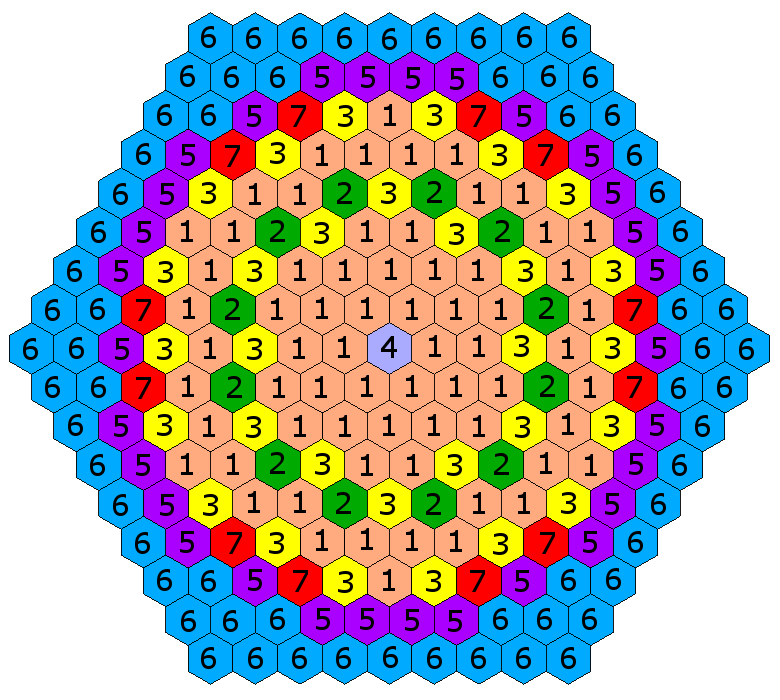
\includegraphics[scale = 0.5] {1.png}
	\caption{Погрешность в $L_2(\omega)$ на равномерной сетке}
	\label{fig:1}
  \end{center}
\end{figure} 
\begin{figure}[htp]
  \begin{center}
    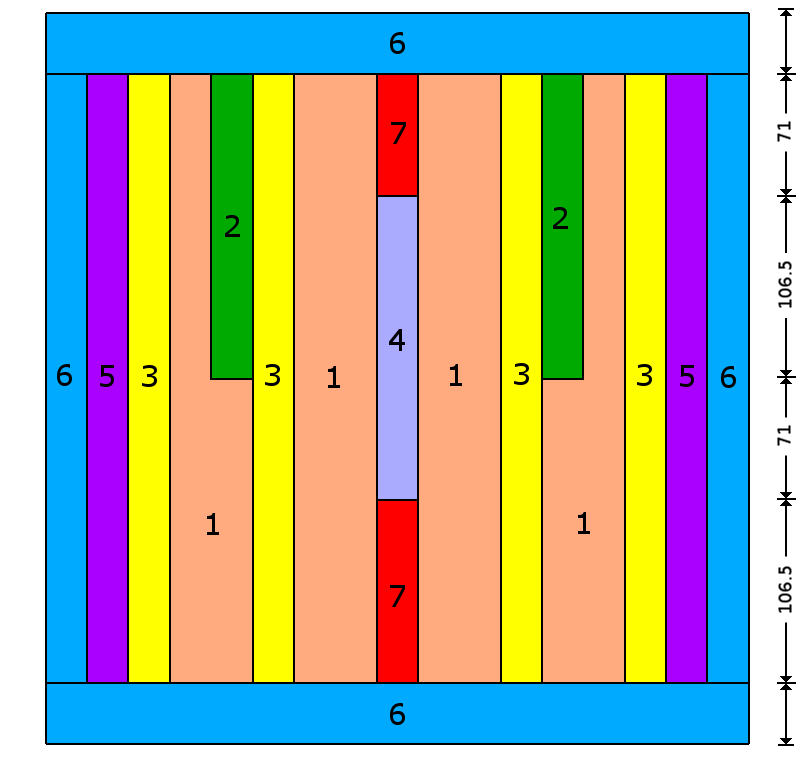
\includegraphics[scale = 0.5] {2.png}
	\caption{Погрешность в $L_\infty (\omega)$ на равномерной сетке}
	\label{fig:2}
  \end{center}
\end{figure} 
\begin{figure}[htp]
  \begin{center}
    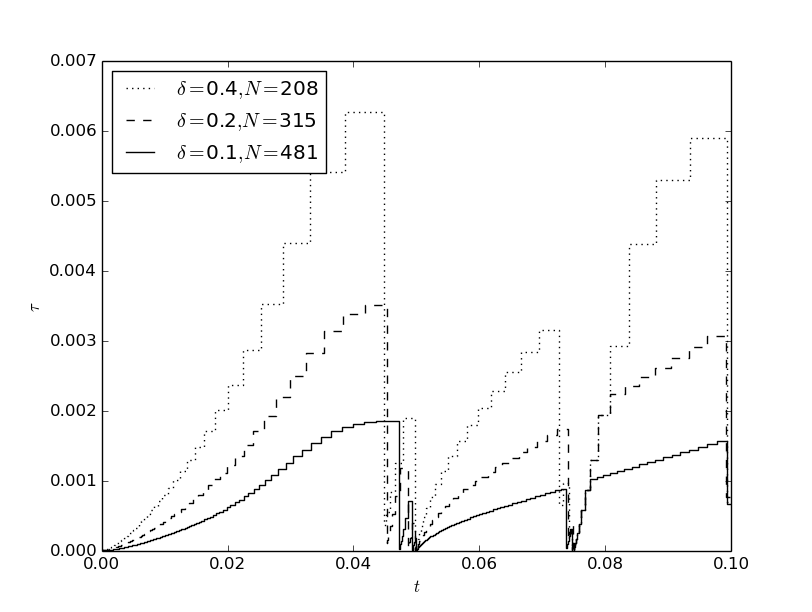
\includegraphics[scale = 0.5] {3.png}
	\caption{Шаги сетки по времени --- $L_2(\omega)$}
	\label{fig:3}
  \end{center}
\end{figure} 
\begin{figure}[htp]
  \begin{center}
    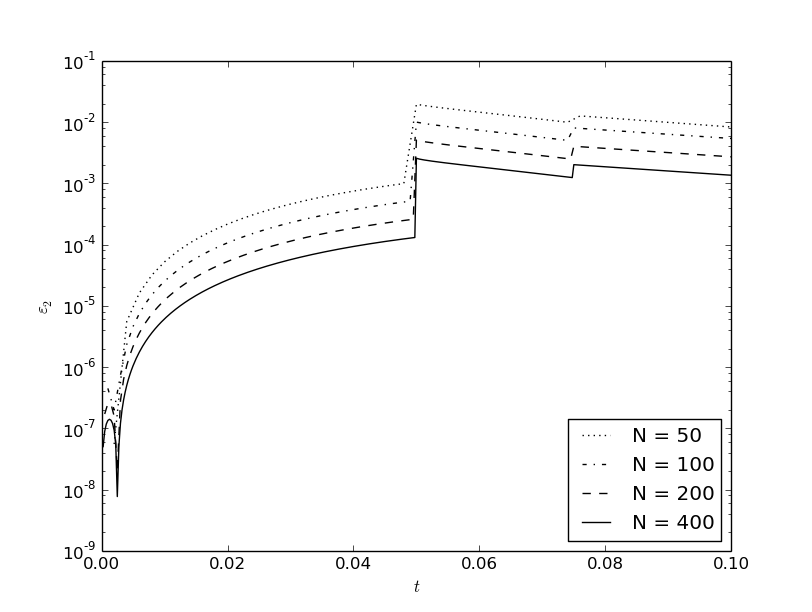
\includegraphics[scale = 0.5] {4.png}
	\caption{Погрешность в $L_2(\omega)$ на неравномерной сетке}
	\label{fig:4}
  \end{center}
\end{figure} 

Уровень погрешности аппроксимации определяется с учетом того, что $T = 0.1$ и приближенное решение
определяется на единичном интервала по $x$, имея амплитуду решения порядка 1.
На фиг.~\ref{fig:3} показаны шаги по времени, которые определяются согласно
(\ref{3.5}), (\ref{3.6}) при использовании нормы $L_2(\omega)$ для оценки погрешности аппроксимации.
Для параметра увеличения шага по времени мы положили $\gamma = 1.5$.
Полученная при этом точность при задании различного уровня погрешности аппроксимации 
представлена на фиг.~\ref{fig:4}. 
Расчет начинается с малого шага и он постепенно увеличивается, в окрестности $t = 0.05$
происходит переход на существенно более мелкий шаг по времени, наблюдается также сброс шага по времени в 
окрестности $t = 0.075$. 
Точность приближенного решения существенно увеличивается при малых временах,
фактически нет потери точности в окрестности разрыва правой части и коэффициента уравнения.

Подобные данные получены при использовании нормы $L_\infty (\omega)$ для
оценки уровня погрешности аппроксимации. Можно сопоставить  фиг.~\ref{fig:5} и  фиг.~\ref{fig:3},
фиг.~\ref{fig:6} и  фиг.~\ref{fig:4}. Видно, что в данном случае начальный (минимальный) шаг должен быть уменьшен
для повышения точности приближенного решения для малых $t$.
Снова наблюдается ярко выраженная смена шага по времени при $t=0.05$ и $t=0.075$ --- при 
разрывах правой части и коэффициента уравнения. Тем самым алгоритм выбора шага по времени
работает при выборе  различных норм для оценки уровня погрешности аппроксимации.

\begin{figure}[htp]
  \begin{center}
    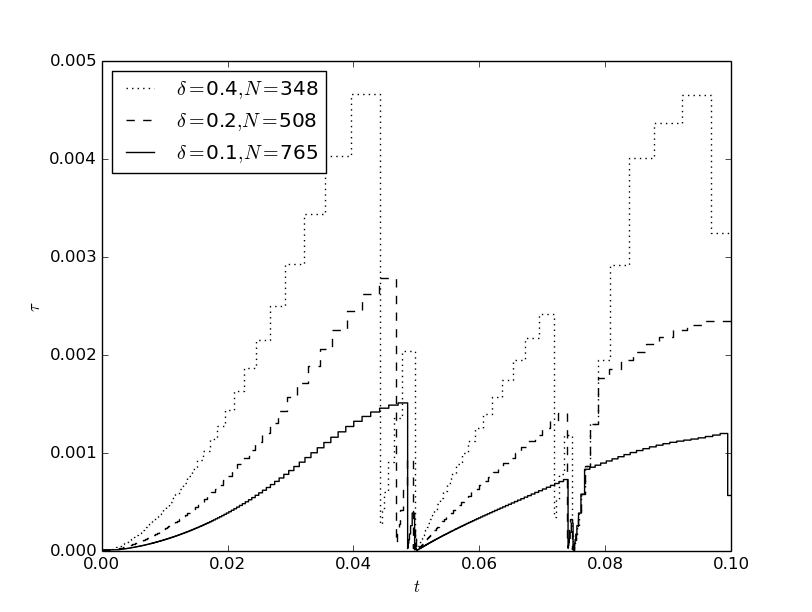
\includegraphics[scale = 0.5] {5.png}
	\caption{Шаги сетки по времени --- $L_\infty (\omega)$}
	\label{fig:5}
  \end{center}
\end{figure} 
\begin{figure}[htp]
  \begin{center}
    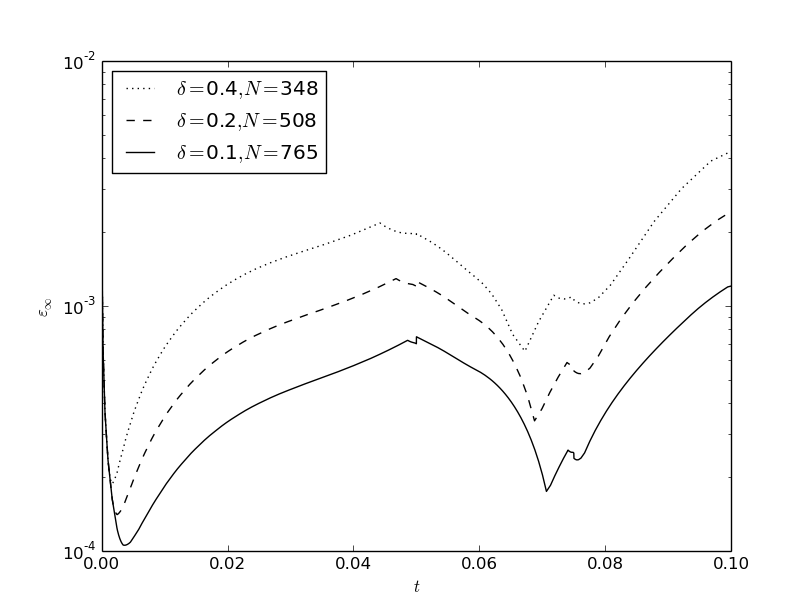
\includegraphics[scale = 0.5] {6.png}
	\caption{Погрешность в $L_\infty (\omega)$ на неравномерной сетке}
	\label{fig:6}
  \end{center}
\end{figure}

Прогнозное решение находиться по явной схеме (\ref{3.3}), которая имеет первый порядок точности, как
и неявная расчетная схема (\ref{2.4}). Мы можем использовать и более точные разностные схемы
для нахождения прогнозного решения. На фиг.~\ref{fig:7} и  фиг.~\ref{fig:8} приведены, например, результаты расчетов 
при использовании трехслойной явной схемы (\ref{4.3}). Сравнение с данными
при использовании явной схемы (\ref{3.3}) (смотри фиг.~\ref{fig:3},~\ref{fig:4}) показывает,
что основные тенденции по выбору шага по времени, достигаемой точности остаются теми же.

\begin{figure}[htp]
  \begin{center}
    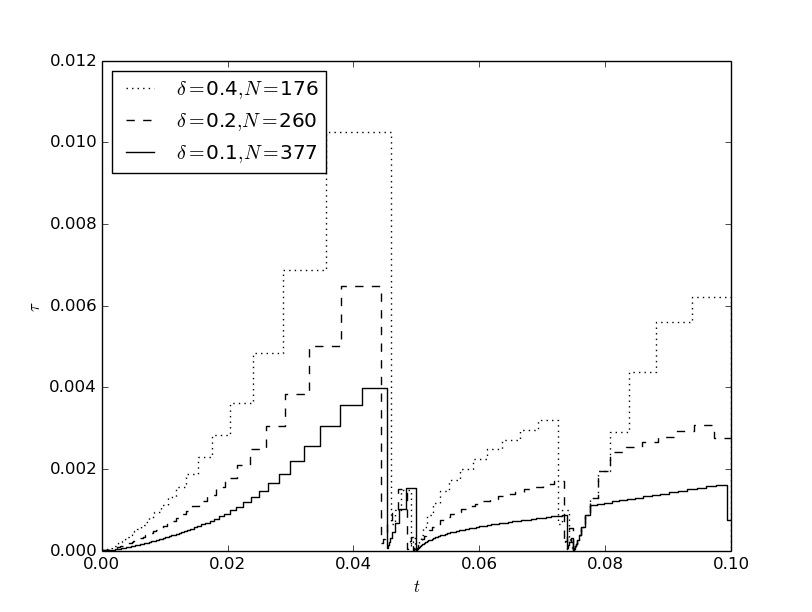
\includegraphics[scale = 0.5] {7.png}
	\caption{Шаги сетки по времени при использовании трехслойной схемы для прогноза}
	\label{fig:7}
  \end{center}
\end{figure} 

\clearpage

\begin{figure}[htp]
  \begin{center}
    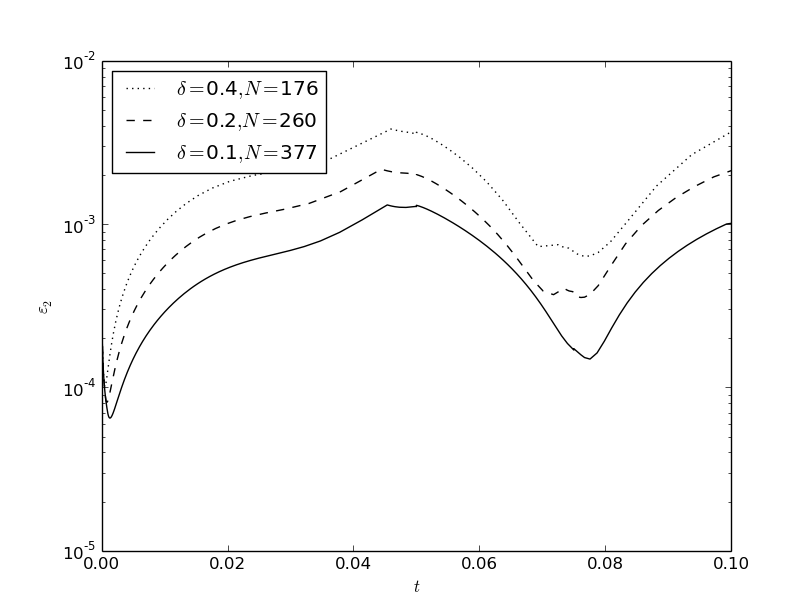
\includegraphics[scale = 0.5] {8.png}
	\caption{Погрешность  при использовании трехслойной схемы для прогноза}
	\label{fig:8}
  \end{center}
\end{figure} 


\begin{figure}[htp]
  \begin{center}
    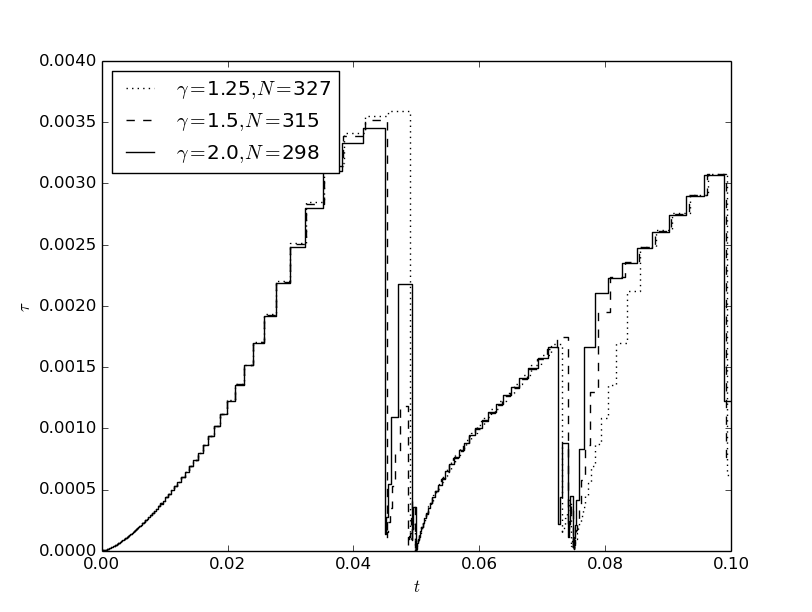
\includegraphics[scale = 0.5] {9.png}
	\caption{Шаги сетки по времени при различных $\gamma$}
	\label{fig:9}
  \end{center}
\end{figure} 
\begin{figure}[htp]
  \begin{center}
    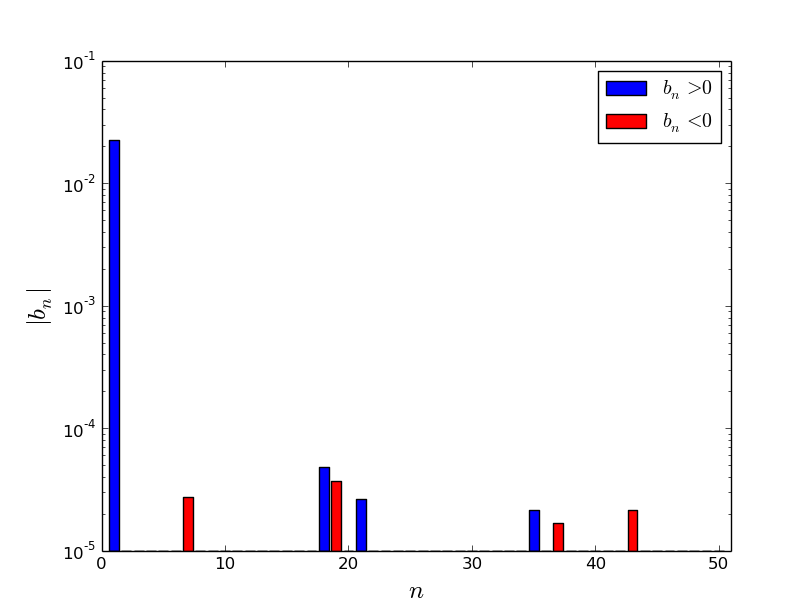
\includegraphics[scale = 0.5] {10.png}
	\caption{Погрешность  при различных $\gamma$}
	\label{fig:10}
  \end{center}
\end{figure} 

 
Среди основных параметром предложенного алгоритма можно отметить
$\gamma$, который связан с выбором прогнозного шага. 
Как показывают данные на фиг.~\ref{fig:9},~\ref{fig:10}
влияние параметра увеличения шага по времени незначительно.

Отдельного внимания заслуживает исследование влияния начальных условий
--- параметра $\sigma$. 
Типичной является ситуация с наличием пограничного слоя, что требует 
использования мелкого шага при небольших временах.
При $\sigma = 1$ мы имеем более благоприятную ситуацию с погрешностью при малых
$t$ (смотри фиг.~\ref{fig:11}). 
Неравномерная сетка и точность приближенного решения приведены 
на  фиг.~\ref{fig:12},~\ref{fig:13}.
В данном случае на начальном участке процесса погрешность малая, что хорошо отрабатывается алгоритмом 
выбора шага по времени. Влияние других параметров задачи ($\lambda$ и $\chi$)
не столь кардинальное.

\begin{figure}[htp]
  \begin{center}
    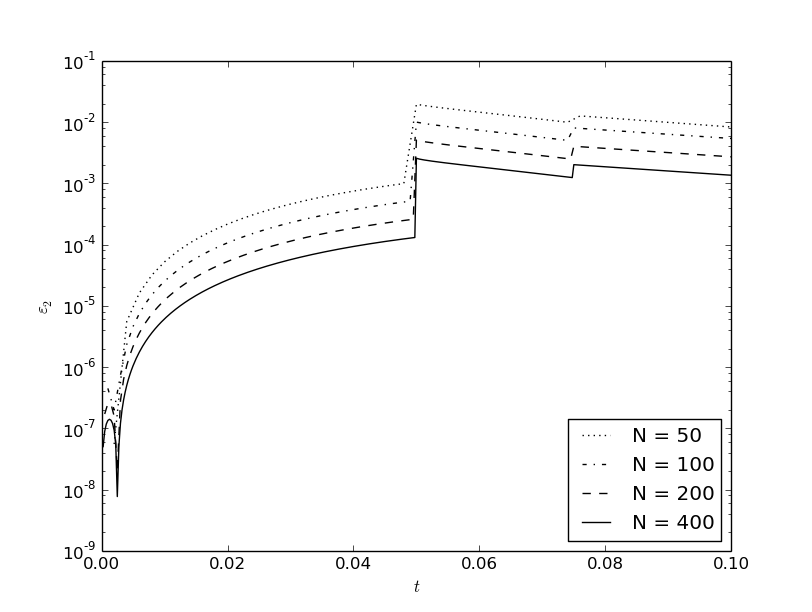
\includegraphics[scale = 0.5] {11.png}
	\caption{Погрешность на равномерной сетке при $\sigma = 1$}
	\label{fig:11}
  \end{center}
\end{figure} 
\begin{figure}[htp]
  \begin{center}
    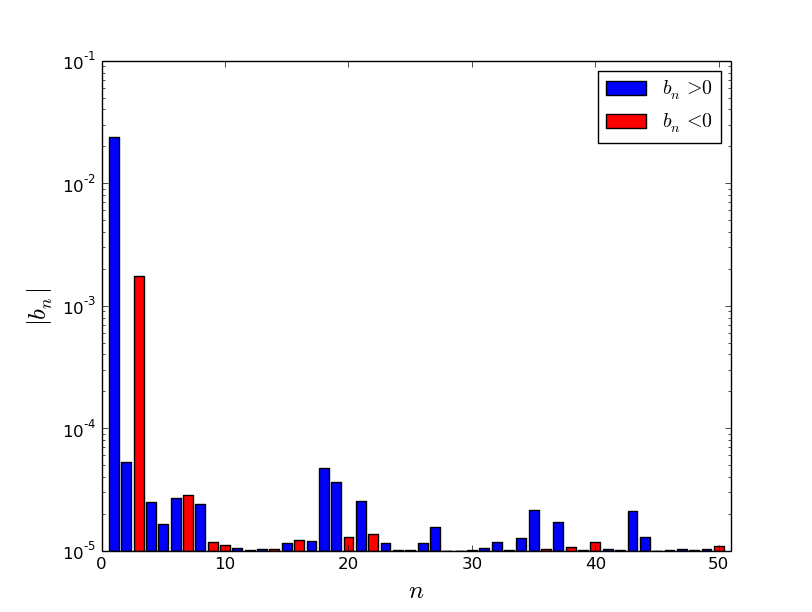
\includegraphics[scale = 0.5] {12.png}
	\caption{Шаги сетки по времени при $\sigma = 1$}
	\label{fig:12}
  \end{center}
\end{figure} 
\begin{figure}[htp]
  \begin{center}
    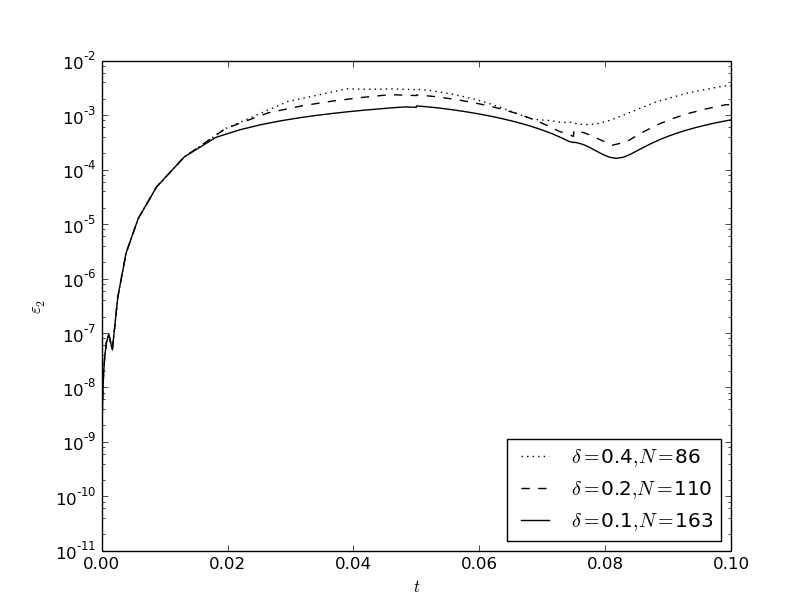
\includegraphics[scale = 0.5] {13.png}
	\caption{Погрешность  при $\sigma = 1$}
	\label{fig:13}
  \end{center}
\end{figure} 
\begin{figure}[htp]
  \begin{center}
    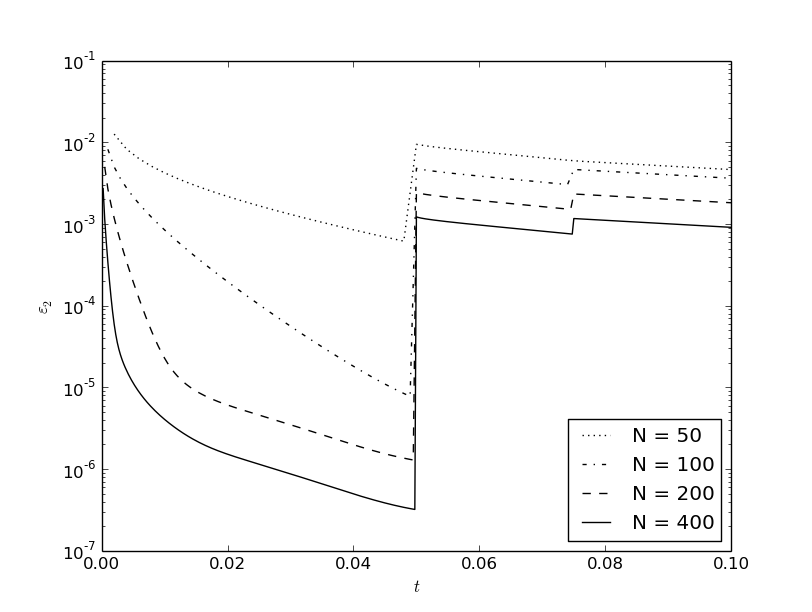
\includegraphics[scale = 0.5] {14.png}
	\caption{Погрешность на равномерной сетке для схемы Кранка--Николсон}
	\label{fig:14}
  \end{center}
\end{figure}
\begin{figure}[htp]
  \begin{center}
    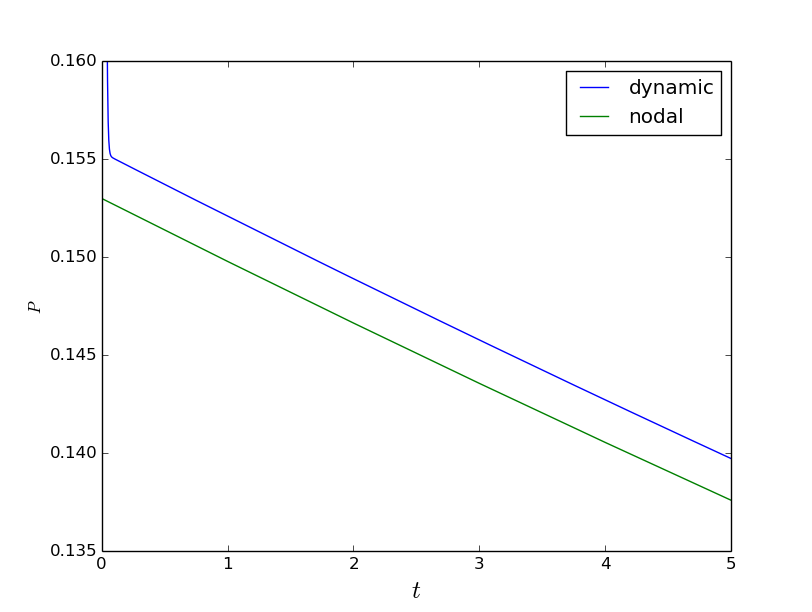
\includegraphics[scale = 0.5] {15.png}
	\caption{Шаги сетки по времени для схемы Кранка--Николсон}
	\label{fig:15}
  \end{center}
\end{figure} 
\begin{figure}[htp]
  \begin{center}
    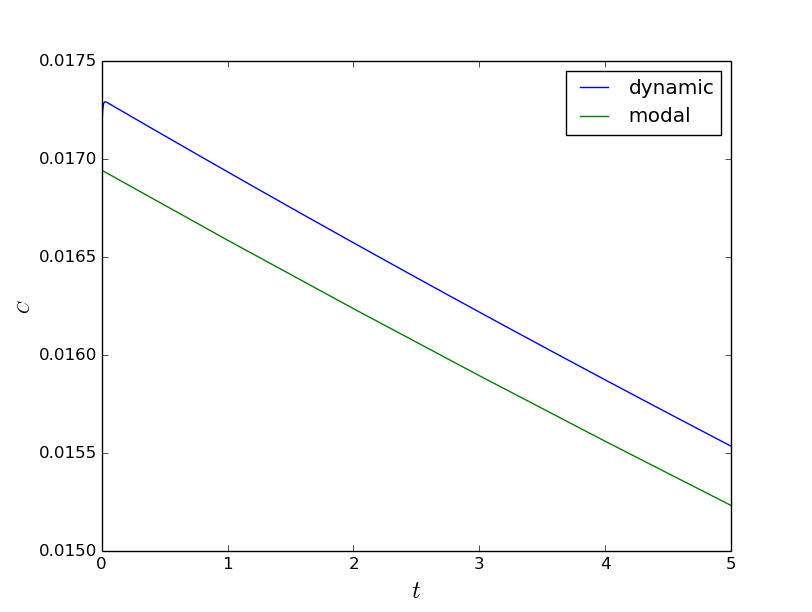
\includegraphics[scale = 0.5] {16.png}
	\caption{Погрешность  для схемы Кранка--Николсон}
	\label{fig:16}
  \end{center}
\end{figure} 
Приведем некоторые результаты расчетов при численном решении модельной
параболической задачи (\ref{5.1})--(\ref{5.3}) с использованием схемы второго порядка (\ref{4.1}).
Точность приближенного решения на равномерной сетке по времени показана фиг.~\ref{fig:14}.
Использовался алгоритм выбора шага по времени (\ref{3.6}), (\ref{4.5}) на основе трехслойной 
схемы (\ref{4.3}). Вырабатываемый шаг по времени показан на фиг.~\ref{fig:15},
точность приближенного решения на неравномерной сетке иллюстрируется фиг.~\ref{fig:16}.
Сравнение фиг.~\ref{fig:15} и фиг.~\ref{fig:14} показывает, что на достаточно 
небольших неравномерных сетках по времени мы получаем решение
с существенно более высокой точностью. 

\clearpage


\begin{thebibliography}{10}

\bibitem{Angermann}
\textit{Knabner P., Angermann~L.} Numerical methods for elliptic and parabolic partial
  differential equations. New York: Springer, 2003.

\bibitem{Ascher}
\textit{Ascher~U.~M.} Numerical methods for evolutionary differential
  equations. Philadelphia: Society for Industrial Mathematics, 2008.

\bibitem{LeVeque}
\textit{LeVeque~R.~J.} Finite difference methods for ordinary and partial
  differential equations. Steady-state and time-dependent problems. Philadelphia: 
Society for Industrial Mathematics, 2007.

\bibitem{Samarskii}
\textit{Samarskii~A.~A.} The theory of difference schemes. New York: Marcel Dekker, 2001.

\bibitem{SamarskiiGulin}
\textit{Самарский А.А., Гулин А.В.} Устойчивость разностных схем. М.: Наука, 1973.

\bibitem{SamarskiiMatusVabishchevich}
\textit{Samarskii~A.~A., Matus P.~P., Vabishchevich P.~N.} Difference schemes with operator factors.
Dordrecht: Kluwer Academic Publishers, 2002.

\bibitem{ascher1998computer}
\textit{Ascher~U.~M.} Computer methods for ordinary differential equations
  and differential-algebraic equations. Philadelphia: Society for Industrial and Applied Mathematics, 1998.

\bibitem{Gear1971}
\textit{Gear~C.~W.} {Numerical initial value problems in ordinary
  differential equations}. New York: Prentice Hall, 1971.

\bibitem{HairerNorsettWanner1987}
\textit{Hairer~E., Norsett S.~P., Wanner G.} Solving ordinary differential equations. I. Nonstiff
  problems. Berlin: Springer, 1987.

\bibitem{bangerth2003adaptive}
\textit{Bangerth~W., Rannacher R.} Adaptive finite element methods for differential
  equations. Basel: Springer, 2003.

\bibitem{moller2011adaptive}
\textit{M{\"o}ller~C.A.} Adaptive finite elements in the discretization of
  parabolic problems. Berlin: Logos-Verlag, 2011.

\bibitem{verfurth2013posteriori}
\textit{Verf{\"u}rth~R.} A posteriori error estimation techniques for finite
  element methods. Oxford: Oxford University Press, 2013.

\bibitem{vabishchevich2015priori}
\textit{Vabishchevich~P.~N.} //  Mathematical Modelling and Analysis. 2015. V.~20. №.~1. P.~94--111.

\bibitem{vabishchevich2015time}
\textit{Vabishchevich~P.~N.} // Finite Difference Methods, Theory and
  Applications. New York: Springer, 2015. P.~96--103.

\bibitem{thomee2010galerkin}
\textit{Thom{\'e}e~V.} Galerkin finite element methods for parabolic
  problems. Berlin: Springer, 2010.

\end{thebibliography}
 

\end{document}

